%学会発表レジュメテンプレート ver. 1.1

%2段落にするためにtwocolumnを追加
\documentclass[uplatex,twocolumn]{jsarticle}
\usepackage[top=20mm,bottom=20mm,left=20mm,right=20mm]{geometry}
\usepackage[T1]{fontenc}
\usepackage{txfonts}
\usepackage{wrapfig}
\usepackage[expert,deluxe]{otf}
\usepackage[dvipdfmx,hiresbb]{graphicx}
%ハイパーリンクに色がつかないようにするため、hidelinksを追加
\usepackage[dvipdfm,hidelinks]{hyperref}
\usepackage{pxjahyper}
%2段落にするために以下を追加
\usepackage{multicol}


\makeatletter
  \renewcommand{\section}{%
    \if@slide\clearpage\fi
    \@startsection{section}{1}{\z@}%
    {\Cvs \@plus.5\Cdp \@minus.2\Cdp}% 前アキ
    {.5\Cvs \@plus.3\Cdp}% 後アキ
    %{\normalfont\Large\headfont\raggedright}}
    {\normalfont\raggedright}}

  \renewcommand{\subsection}{\@startsection{subsection}{2}{\z@}%
    {\Cvs \@plus.5\Cdp \@minus.2\Cdp}% 前アキ
    {.5\Cvs \@plus.3\Cdp}% 後アキ
    %{\normalfont\large\headfont}}
    {\normalfont}}

  \renewcommand{\subsubsection}{\@startsection{subsubsection}{3}{\z@}%
    {\Cvs \@plus.5\Cdp \@minus.2\Cdp}%
    {\z@}%
    %{\normalfont\normalsize\headfont}}
    {\normalfont}}
    
  %2段落で画像貼り付けをするために以下を追加    
  \newenvironment{figurehere}
    {\def\@captype{figure}}
    {}      
    
\makeatother
%ここから上を編集する必要はない.





\title{\vspace{-14mm}研究タイトル \footnotemark[0]}
\author{氏名 \footnotemark[2] \\ 千葉工業大学 社会システム科学部 プロジェクトマネジメント学科\footnotemark[2]}
\date{}%日付を入れる必要はない.
\pagestyle{empty}%ページ番号は振らない.
\begin{document}
%タイトルを1段落にするために以下を追加
\twocolumn[
	\maketitle
]

%脚注の追加をするために以下を追加
\begingroup
\def\thefootnote{\fnsymbol{footnote}}
\footnotetext[0]{英語の研究タイトル}
\footnotetext[2]{英語の氏名・Department of Project Management, Social System Sciences, Chiba Institute of Tchnology}
\endgroup




\section{研究の背景}

矢吹研究室では課題研究のレジュメは\LaTeX で書くことになっている.その理由は2つある.

第1の理由は,文書自体や参考文献の形式を厳密に統一したいということである.正しい形式で書かれることは,文章が読みやすくなることの必要条件である.正しい形式で書くためには,正しい形式(参考文献を挙げる際の形式も含む)とはどのようなものかを知らなければならない.\LaTeX の基本機能を学ぶことでそれを意識するようになることが期待できる.

第2の理由は,図表や参考文献,索引の参照・被参照関係の管理を自動化することである.技術的な文書では,図表や参考文献には番号やラベルを付けて参照することが多いが,\LaTeX には,それらを自動的に管理する機能がある.ある程度の長さの文書には,索引が付くことが望ましいが,\LaTeX には,指定した語を自動的に索引にまとめる機能もある.それらを活用することによって,文書作成の効率を上げることが期待できる.





\section{研究の目的}

\LaTeX の基本的な使い方をまとめ,周知することを目的とする.





\section{プロジェクトマネジメントとの関連}

プロジェクトにおいては,厳密に定義された形式に従って文書を作成することが求められることがある.その際,プロジェクトのメンバには,定義された文書の形式を理解する素養が求められる.\LaTeX は,そのような素養を身につけるための最適な題材の一つであろう.





%\begin{wrapfigure}[行数]{r}{幅}%行数はオプションだが,調整しないとうまくいかない.
\begin{wrapfigure}[11]{r}{5cm}
\vspace*{-\intextsep}
%\includegraphics[width=図の幅,clip]{ファイル名}\label{参照用ラベル}
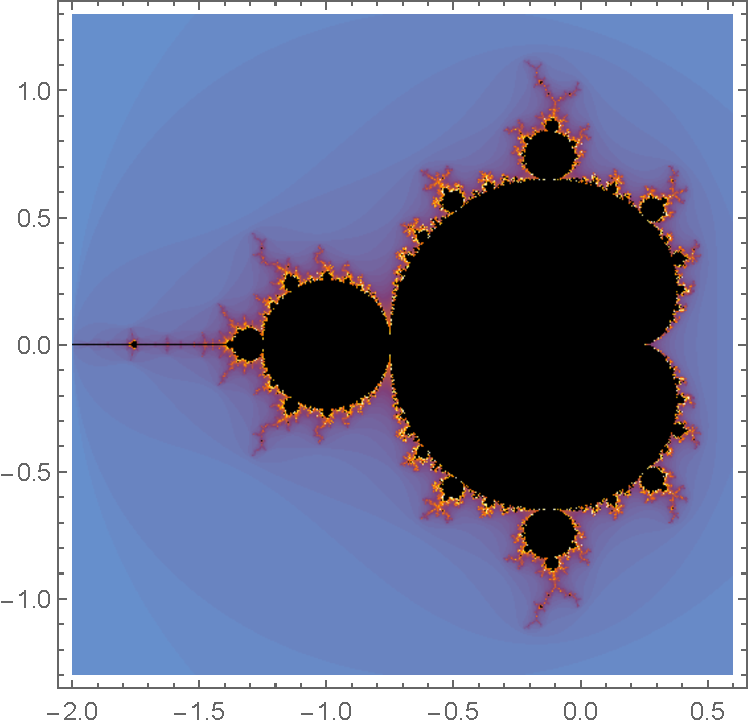
\includegraphics[width=5cm,clip]{figure.pdf}
\caption{図の挿入例}\label{サンプル図}
\end{wrapfigure}

\section{研究の方法}

\subsection{\LaTeX 原稿の書き方}

研究室専用のテンプレートファイル(\verb|draft.tex|と\verb|biblio.bib|)を用意する.課題研究のレジュメを作成する際は,この2つのファイルをコピーし,編集すればよい.いずれもテキストファイルだから,テキストエディタで編集すればよいが,文献ファイルはJabRefで編集する方が簡単だろう(JabRefを利用するためにはJavaの実行環境が必要である.Options, Preferences, Appearance, Set table fontでフォントを変更する必要もある).



\subsubsection{図}

図を用いる場合は,それが描かれたPDFファイルを用意し,この文書のような方法(ソースを参照)で文書に埋め込めばよい.\verb|\label|と\verb|\ref|を使うようにすれば,図\ref{サンプル図}のような参照番号は自動的に管理される.



%\begin{wraptable}[行数]{r}{幅}%行数はオプションだが,調整しないとうまくいかない.
\begin{wraptable}[5]{r}{5cm}
\vspace*{-\intextsep}
\caption{表の挿入例}\label{サンプル表}
\begin{tabular}{cc}
\hline
文字 & コードポイント \\
\hline
\UTF{005C} & U+005C\\
\UTF{00A5} & U+00A5\\
\hline
\end{tabular}
\end{wraptable}

\subsubsection{表}

表を用いる場合は,この文書のような方法(表\ref{サンプル表}の部分のソースを参照)で文書に埋め込めばよい(表の詳細は文献\cite{okumura2013}を参照).複雑な表は,Excel上で作成した表を\LaTeX 形式に変換するツールを使って書くといいだろう.表の参照番号については,図の場合と同様である.



\subsubsection{参考文献の参照方法}

参考文献は文献ファイル(この文書では\verb|biblio.bib|)に記述し,\verb|\cite|で参照する.例:データベースのための問い合わせ言語SQLで数独を解く方法が提案されている\cite{yabuki2011}.このように参照すると,参考文献リストに自動的に登録される.文献の種類には,雑誌論文\cite{yabuki2011}や会議録論文\cite{yabuki2013},卒業論文\cite{kubo2014},書籍\cite{okumura2013},ウェブサイト\cite{self}などがある.文献の種類によって必要な項目が異なるため,\verb|biblio.bib|を見て確認すること.

細かい注意:\LaTeX の命令の先頭は「\UTF{005C}\hspace{-0.5zw}」だが,Webなどの資料ではそれが「\UTF{00A5}\hspace{-0.5zw}」になっていることがある.テキストエディタでは,VLゴシックのような「\UTF{005C}\hspace{-0.5zw}」と「\UTF{00A5}\hspace{-0.5zw}」を区別できるフォントを使うといい.





\subsection{\LaTeX 原稿の処理方法}

原稿の作成に必要な作業は以下の通りである.

\begin{enumerate}
\item TeXLiveをインストールする.
\item SumatraPDFをインストールする(Acrobatはファイルをロックするから使いにくい).
\item 原稿(\verb|draft.tex|や\verb|.bib|,\verb|.pdf|など)を用意する.(ここでは,作業ディレクトリを「\verb|C:/work|」とする.)
\item コマンドプロンプトで「\verb|C:|\UTF{23CE}\verb|cd /work|\UTF{23CE}」などとして作業ディレクトリに移動する.
\item 「\verb|uplatex -shell-escape draft|」で\LaTeX 処理,「\verb|dvipdfmx draft|」でPDF作成をするのが基本.参考文献リストが変わったときは「\verb|upbibtex draft|」を1回,参照情報が変わったときは「\verb|uplatex -shell-escape draft|」を2回実行する.\verb|build.bat|を使ってもよい.途中でエラーで止まったら,「\verb|q|\UTF{23CE}」やCtrl-Cで終了する.
\item \verb|draft.pdf|をSumatraPDFで開いて結果を確認する.
\end{enumerate}





\section{現在の進捗状況}

研究室専用のテンプレートファイル(\verb|draft.tex|と\verb|biblio.bib|)を作成した.



\section{今後の計画}

以下のように研究を進める計画である.

\begin{enumerate}
\item \LaTeX の基本的な使い方を確認する.(まずはこのPDFファイルを再現できることを確認するといい.)
\item 研究テーマを決め,研究する.
\item レジュメとポスターを書き,pull requestする.(やり方は先輩に習うこと.)\label{pull request}
\item 矢吹がファイルをマージすれば終了.マージされなかったら\ref{pull request}に戻る.
\end{enumerate}

\bibliographystyle{junsrt}
\bibliography{biblio}%「biblio.bib」というファイルが必要.

\end{document}
